\section{Evaluation}
\label{sec:eval}

\subsection{Setup}
All measurements ran on one laptop (Intel Core i7-12700H, 14 cores/20 threads, 25.4\,GB RAM, Windows~11) with FFmpeg~8.0.1 (x264 core~165), Node.js~22.20 and snarkjs~0.7.6. Sources are nine Xiph CIF sequences~\cite{xiph_media} (akiyo, city, coastguard, container, deadline, football, two foreman variants, hall\_monitor), 30 frames each, encoded at their native $352\times288$ and Lanczos-upscaled to $640\times480$ and $1280\times960$ (upscaled sequences test scaling, not native high-resolution content). The benchmark encoder is x264 \emph{ultrafast}/zerolatency, Constrained Baseline, QP~22 for P frames (the I-slice QP is 19), all-intra, one slice per IDR; this preset uses only Intra16$\times$16 MBs and no deblocking. Each case embeds a 68-byte message with its proof (payload 201\,B, 1{,}632 frame bits) at the default cap of 64 bits per IDR, i.e.\ into 26 of the 30 IDRs, under a fresh stego key and an 8-camera registry. Wall times include process start-up (Node.js for snarkjs).

\subsection{Functional results}
All 27 cases passed every acceptance check: native capacity scan, embedding, strict FFmpeg decoding (\texttt{-xerror}), blind extraction of the exact payload, a video-bound proof verified against the registry root with the digest recomputed from the stego file, rejection under a wrong key, and zero sign changes outside the keyed schedule (checked position by position). The stego file has exactly the size of the cover in all 27 cases. A separate end-to-end run on 300 CIF frames passed five of five trials.

\subsection{Embedding quality}
Table~\ref{tab:quality} reports PSNR-Y and SSIM~\cite{wang2004ssim} per frame, comparing the clean decode of the cover with the decode of the stego stream (incremental embedding distortion), and from the original source (encoding plus embedding). About half of the 1{,}632 scheduled signs change (808--823 on average), i.e.\ about 31 per carrying frame. No frame falls below the common 40\,dB reference. The encoder's own loss dominates: on average, cover$	o$stego PSNR is 12--15\,dB higher than source$	o$stego PSNR.

\begin{table}[t]
\centering
\caption{Per-frame quality over the 26 carrying frames of 9 sequences per resolution.}
\label{tab:quality}
\setlength{\tabcolsep}{4pt}
\begin{tabular}{@{}lccc@{}}
\toprule
& CIF & $640\times480$ & $1280\times960$ \\
\midrule
Cover$\to$stego PSNR-Y, min [dB] & 46.71 & 44.03 & 44.72 \\
Cover$\to$stego PSNR-Y, mean [dB] & 57.44 & 59.69 & 62.64 \\
Cover$\to$stego SSIM, min & 0.99871 & 0.99895 & 0.99960 \\
Source$\to$stego PSNR-Y, min [dB] & 41.48 & 41.62 & 42.94 \\
Source$\to$stego PSNR-Y, mean [dB] & 45.57 & 46.43 & 48.11 \\
Changed signs per case (mean) & 808 & 823 & 816 \\
Candidates per case (mean) & 149{,}374 & 420{,}193 & 1{,}287{,}323 \\
\bottomrule
\end{tabular}
\end{table}

\subsection{Validating the distortion model}
\label{sec:eval-distortion}

We test the model of Section~\ref{sec:distortion} in three experiments (scripts and raw data in the artifact): (B)~single flips decoded in isolation, which measure the direct energy and the gain of individual carriers; (A)~the 27 benchmark encodes, which measure frame-level distortion with $\sim$22 luma flips per frame; and (C)~an inverse check that sets the cap from a target PSNR, embeds and measures.

\textbf{Experiment B: single flips.} We encoded the first frame of \emph{foreman} and \emph{city} (CIF) with two x264 configurations---\emph{ultrafast} (Intra16$\times$16 only, deblocking off; the benchmark encoder) and \emph{medium} (Intra4$\times$4 and Intra16$\times$16, deblocking on)---at QP~22, 28 and 34 (I-slice QP 19, 25, 31), sampled 100 candidates per encode (1{,}200 in total, skipping the rare carriers whose flip would add or remove an emulation-prevention byte), flipped each one alone and decoded with and without the loop filter.

\emph{Direct energy.} For all 385 sampled Intra4$\times$4 luma carriers, the change of the flipped block's own samples in the unfiltered decode equals, sample for sample, the change of the residual computed from Eqs.~\eqref{eq:dequant} and~\eqref{eq:inverse} with rounding; the decoder adds nothing else to the block. The ratio of that exact energy to the model value $4\Qs^2$ has median $1.012$ and mean $1.022$ (5th--95th percentile 0.95--1.19; small residuals are the most affected by rounding), and the pre-rounding factor $\kappa$ of the sampled positions lies in $[1.000,1.056]$, as Lemma~\ref{lem:flip} states.

\emph{Gains.} Table~\ref{tab:single} summarizes $G$. Three observations matter for the model. First, $G$ does not depend on QP (luma mean 6.6, 7.4, 6.0 for ultrafast and 38.4, 33.3, 34.0 for medium at the three QPs), so distortion scales as $\Qs^2$, i.e.\ by 6\,dB per six QP steps. Second, the gain is heavy-tailed: the median carrier barely propagates ($G\approx1$--$2$), but single luma gains reach 309 (ultrafast) and 2{,}187 (medium), and the 10\% largest gains account for 80\% (ultrafast) and 84\% (medium) of the total energy. Third, the encoder configuration matters more than anything else: the mean luma gain is 6.6 with Intra16$\times$16 only and 35.2 with Intra4$\times$4, whose nine directional modes chain many blocks. Deblocking changes the mean luma gain by about 1\% (35.6 without, 35.2 with), so drift through intra prediction, not filtering, is the propagation mechanism.

\begin{table}[t]
\centering
\caption{Single-flip propagation gain $G$ by carrier category (experiment B; $n$ flips, mean, median, 90th percentile).}
\label{tab:single}
\setlength{\tabcolsep}{4pt}
\begin{tabular}{@{}lrrrr@{\quad}rrrr@{}}
\toprule
& \multicolumn{4}{c}{ultrafast} & \multicolumn{4}{c}{medium} \\
Category & $n$ & mean & med. & p90 & $n$ & mean & med. & p90 \\
\midrule
Luma AC / 4$\times$4 & 352 & 3.7 & 1.04 & 5.7 & 395 & 35.4 & 2.1 & 52.9 \\
LumaDC & 38 & 33.8 & 4.9 & 64.4 & 5 & 16.3 & 12.6 & 31.6 \\
ChromaAC & 173 & 9.2 & 1.12 & 11.9 & 146 & 4.4 & 1.06 & 5.4 \\
ChromaDC & 37 & 23.9 & 7.1 & 65.3 & 54 & 30.5 & 11.4 & 102.2 \\
\midrule
All luma & 390 & 6.6 & 1.05 & 7.8 & 400 & 35.2 & 2.2 & 47.5 \\
\bottomrule
\end{tabular}
\end{table}

\begin{figure}[t]
\centering
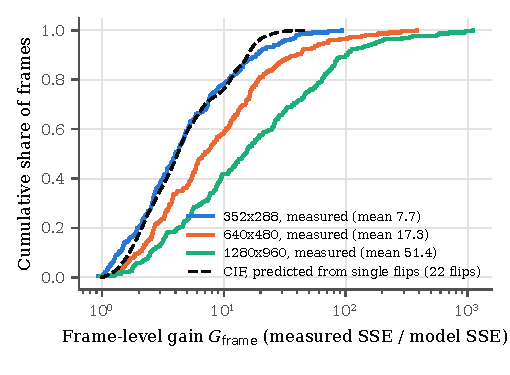
\includegraphics[width=\linewidth]{figures/frame_gain_cdf.pdf}
\caption{Frame-level gain of the 702 benchmark frames with luma flips (experiment A), and its prediction for CIF from single flips alone (experiment B, 22 independent draws per frame).}
\label{fig:framegain}
\end{figure}

\begin{figure*}[t]
\centering
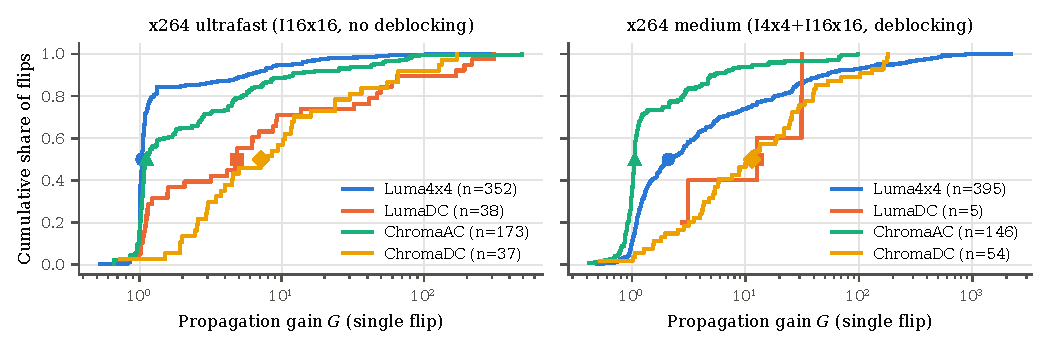
\includegraphics[width=\textwidth]{figures/gain_cdf.pdf}
\caption{Distribution of single-flip gains per carrier category for the two encoder configurations (markers: medians).}
\label{fig:gaincdf}
\end{figure*}

\textbf{Experiment A: sequences.} For each of the 810 frames of the benchmark we located every changed bit in the bitstream, classified it with the parser, summed the model energy $4\Qs^2$ per plane and compared it with the measured SSE between the cover and stego decodes. Table~\ref{tab:sequence} reports the frame-level gain. Its \emph{mean} (the ratio of total measured to total predicted energy) is the quantity Eq.~\eqref{eq:forward} needs; for CIF it is 7.7, close to the single-flip mean of 6.6 measured on different frames in experiment B. More strikingly, Fig.~\ref{fig:framegain} shows that drawing 22 single-flip gains at random reproduces the whole distribution of the CIF frame gains up to its 90th percentile (median 4.17 predicted vs.\ 4.00 measured); the measured upper tail is heavier (95th percentile 28.6 vs.\ 18.4), because carriers of the same frame share its content and are not independent. The gain grows with resolution (7.7, 17.3, 51.4). Our upscaled sequences contain large smooth regions, where Intra16$\times$16 prediction carries a change across many MBs; native high-resolution content may behave differently, and calibrating $\bar G$ per resolution and encoder is necessary.

Because a frame's distortion is dominated by its few high-gain carriers, the model predicts the \emph{distribution} of frame PSNR, not individual frames: with the per-resolution mean gain, the per-frame PSNR error has a mean absolute value of 4.1--6.7\,dB and a correlation of only 0.19--0.35 with the measurement (leave-one-sequence-out errors are the same to 0.05\,dB, so the gain does not overfit a sequence).

\begin{table}[t]
\centering
\caption{Frame-level gain in the 27-encode benchmark (experiment A, ultrafast, 64 bits per IDR).}
\label{tab:sequence}
\setlength{\tabcolsep}{4pt}
\begin{tabular}{@{}lccc@{}}
\toprule
& CIF & $640\times480$ & $1280\times960$ \\
\midrule
Frames with luma flips & 234 & 234 & 234 \\
Luma flips per frame & 22.0 & 22.7 & 22.9 \\
Mean gain $\bar G$ & 7.7 & 17.3 & 51.4 \\
Frame gain, median & 4.0 & 7.0 & 15.2 \\
Frame gain, 95th pct. & 28.6 & 65.8 & 173.8 \\
Measured PSNR-Y, median [dB] & 57.9 & 60.1 & 62.7 \\
Per-frame error, MAE [dB] & 4.1 & 5.1 & 6.7 \\
\bottomrule
\end{tabular}
\end{table}

\textbf{Experiment C: the inverse.} We encoded 30 frames of \emph{foreman} (CIF) with both configurations, computed the cap with Eq.~\eqref{eq:inverse-cap} for $T=40$, 45 and 50\,dB under three choices of the gain, embedded a random payload filling the capacity, and repeated each setting with five independent keys and payloads (145 fully loaded frames per setting): (i)~\emph{expected}, the mean single-flip gain of experiment B, which makes the expected frame energy equal to the budget; (ii)~\emph{p95-MC}, the 95th percentile of the frame gain obtained by Monte Carlo from single flips; (iii)~\emph{p95-sequence} (ultrafast only), the 95th percentile of the measured CIF frame gains of experiment A. The single-flip gains are pooled over both sources and all three QPs, which Table~\ref{tab:single} justifies for QP (the QP-19 subset has mean luma gain 6.6 and 38.4 against 6.6 and 35.2 pooled); the pool contains the first frame of \emph{foreman} but none of the other 29 test frames. The third policy uses data that include these frames' sequence. A cap at or above the number of candidates in an IDR (about 650 for ultrafast and 460 for medium here) saturates: every candidate is used and the target no longer controls anything.

\begin{table}[t]
\centering
\caption{Inverse check (experiment C): gain used, cap, share of frames with PSNR-Y $\ge T$ and 5th-percentile PSNR-Y [dB]; $^{s}$: cap at or above the candidate count of at least 97\% of the frames' IDRs (saturated).}
\label{tab:inverse}
\footnotesize\setlength{\tabcolsep}{3.2pt}
\begin{tabular}{@{}llrrrrr@{}}
\toprule
Encoder & Policy & $G$ & $T$ & cap & $\ge T$ & p05 \\
\midrule
\multirow{6}{*}{medium} & expected & 35.2 & 45 & 200 & 61\% & 40.2 \\
& expected & 35.2 & 50 & 63 & 70\% & 45.1 \\
& p95-MC & 63.4 & 40 & 351 & 86\% & 38.3 \\
& p95-MC & 102.4 & 45 & 68 & 88\% & 43.2 \\
& p95-MC & 140.1 & 50 & 15 & 86\% & 43.6 \\
& expected & 35.2 & 40 & 634$^{s}$ & 75\% & 37.3 \\
\midrule
\multirow{5}{*}{ultrafast} & expected & 6.6 & 50 & 311 & 46\% & 44.3 \\
& p95-MC & 15.8 & 50 & 130 & 80\% & 47.4 \\
& p95-seq. & 28.6 & 45 & 228 & 92\% & 43.7 \\
& p95-seq. & 28.6 & 50 & 72 & 91\% & 48.8 \\
& all three & -- & 40 & $\ge$721$^{s}$ & 99\% & 41.5 \\
\bottomrule
\end{tabular}
\end{table}

\begin{figure*}[t]
\centering
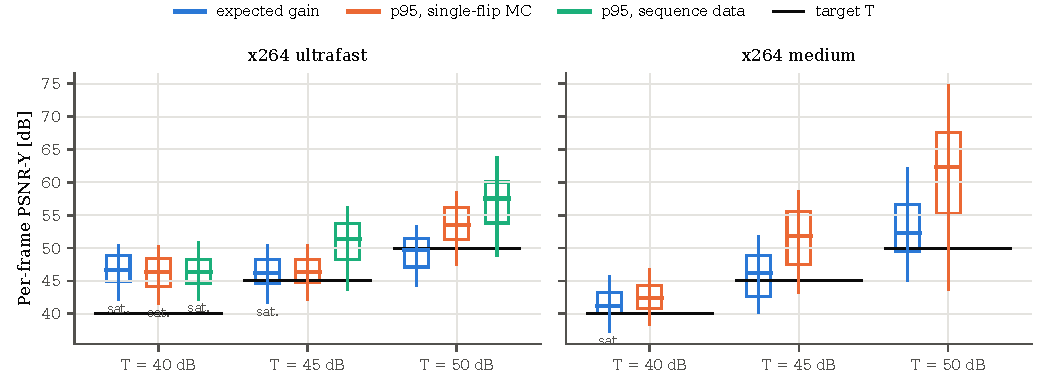
\includegraphics[width=0.8\textwidth]{figures/inverse_check.pdf}
\caption{Per-frame PSNR-Y for caps derived from a target $T$ (boxes: quartiles; whiskers: 5th--95th percentiles; 145 frames per box).}
\label{fig:inverse}
\end{figure*}

Table~\ref{tab:inverse} and Fig.~\ref{fig:inverse} give the outcome. The \emph{expected} policy places the median frame near the target, as intended (46--70\% of frames reach $T$). A percentile policy trades capacity for reliability: with the Monte Carlo percentile 80--88\% of frames reach $T$, short of the nominal 95\% for the reason seen in Fig.~\ref{fig:framegain} (correlated carriers within a frame), while the percentile measured on sequences reaches 91--92\%. Content is the other factor: the single-flip mean luma gain of \emph{foreman} alone at QP~19 is about twice the pooled value (12.9 vs.\ 6.6 for ultrafast, 70 vs.\ 35 for medium, $n\approx48$ each), so a gain calibrated on other content under-protects a sequence that propagates more. In every non-saturated setting the 5th percentile stays within 6.5\,dB below the target, and the cap moves in the direction and by the amount the model predicts: from $T=45$ to $50$\,dB the cap shrinks by $10^{0.5}\approx3.2\times$ under the expected policy (200 to 63, 983 to 311). Saturation itself is informative: at the benchmark's QP the ultrafast stream cannot drop below about 41.5\,dB at its 5th percentile even when every candidate is used.

\textbf{What the data suggest for carrier selection.} Since a tenth of the carriers produces four fifths of the distortion, excluding high-gain carriers is worth more than reducing the payload. The single-flip data show which invariant features predict the gain. In the medium configuration, low-frequency trailing ones (coefficient positions with $i+j\le1$) have mean gains of 84--92 against 1.6 at $i+j=6$, because low-frequency basis functions change the right column and bottom row from which later blocks predict. In both configurations, carriers in the top third of the picture have mean gains of 13.9 (ultrafast) and 65.6 (medium), against 2.2 and 6.1 in the bottom third, because more blocks are predicted from them. Restricting a random schedule to bottom-third carriers would reduce the expected energy by 4.8\,dB (ultrafast) and 7.6\,dB (medium) according to these averages, and excluding DC paths by 2.5\,dB (ultrafast). These are projections from single-flip averages, not end-to-end measurements; the cost-aware schedule they motivate keeps the receiver-computability constraint of Section~\ref{sec:distortion}.


\subsection{Sign statistics}
Over all candidate signs of a case, the share of negative trailing ones is $0.504$ before and after embedding; the two-proportion $z$-statistic is at most $0.223$ in absolute value over the 27 cases, far from the 1.96 threshold of a 5\% test. This is a first-order indicator only (Section~\ref{sec:discussion}).

\subsection{Performance}
Table~\ref{tab:zkp} compares Groth16 and PLONK on the same R1CS and witness; both verify a correct proof and reject a tampered public input. Groth16's 129-byte proof is what makes the covert channel practical: snarkjs serializes a PLONK proof as 2.25\,KB of JSON, which would need about 290 IDRs at the default cap, and even a compact binary encoding is several times larger than 129\,B. Table~\ref{tab:e2e} gives the end-to-end stages for 300 CIF frames. Native costs scale with the number of parsed IDRs: the median capacity scan takes 52, 220 and 770\,ms per IDR at the three resolutions, embedding 61, 245 and 891\,ms per carrying IDR, and the digest, which parses the 26 carrying IDRs, 1.6, 6.4 and 22.6\,s. Parsing, not proving, bounds throughput at high resolution; the parser is single-threaded and unoptimized.

\begin{table}[t]
\centering
\caption{Proof systems on the \texttt{camera\_video} circuit (8{,}737 constraints, 3 public inputs).}
\label{tab:zkp}
\begin{tabular}{@{}lcc@{}}
\toprule
& Groth16 & PLONK \\
\midrule
Trials & 5 & 3 \\
Prove [s] & 1.52--1.60 & 21.5--23.3 \\
Verify [s] & 0.91--1.01 & 0.90--0.94 \\
Proof size & 129\,B (compressed) & 2.25\,KB (JSON) \\
Peak prover RSS [MB] & 695 & 864 \\
Setup & circuit-specific (Phase 2) & universal SRS, 3.2\,s \\
Proving key & 4.2\,MB & 30.1\,MB \\
\bottomrule
\end{tabular}
\end{table}

\begin{table}[t]
\centering
\caption{End-to-end stages, 300 CIF frames, 5 trials (median, ms).}
\label{tab:e2e}
\begin{tabular}{@{}lr@{\qquad}lr@{}}
\toprule
\multicolumn{2}{@{}c}{Sender} & \multicolumn{2}{c@{}}{Receiver} \\
\midrule
Cover digest & 511 & Extract & 535 \\
Groth16 prove & 1{,}774 & Digest + verify & 1{,}448 \\
Embed & 500 & Strict decode & 150 \\
\textbf{Total} & \textbf{2{,}779} & \textbf{Total} & \textbf{1{,}989} \\
\bottomrule
\end{tabular}
\end{table}

\subsection{Attack matrix}
Table~\ref{tab:attacks} lists the attacks run through the service's verify job on the end-to-end stream. Only the untouched stream is accepted. Notably, flipping a sign that does not carry the frame---in an IDR that does carry it---is rejected through the digest, and so is the same valid payload embedded into another video; a camera that builds its own registry produces a proof that verifies against its own root but not against the trusted one.

\begin{table}[t]
\centering
\caption{Attack matrix (verify job outcome and reason).}
\label{tab:attacks}
\footnotesize
\begin{tabular}{@{}ll@{}}
\toprule
Case & Result (rejection reason) \\
\midrule
Untouched stego stream & accepted \\
Wrong stego key & \texttt{payload\_not\_found} \\
Flip a scheduled carrier sign & \texttt{malformed\_proof\_payload} \\
Flip non-carrier sign, carrier IDR & \texttt{proof\_invalid} \\
Flip a sign in a later frame & \texttt{proof\_invalid} \\
Drop the first IDR & \texttt{payload\_not\_found} \\
Truncate to half & \texttt{proof\_invalid} \\
Re-encode (transcode) & \texttt{payload\_not\_found} \\
Swap the message & \texttt{proof\_invalid} \\
Camera outside the registry & \texttt{proof\_invalid} \\
Replay into another video & \texttt{proof\_invalid} \\
\bottomrule
\end{tabular}
\end{table}
